% ============================================== %
%
% 
%
%% ============================================== %
\chapter{Results and Discussion}
    \section{Evaluation of Movement Classification Models}
        % \subsection{Validation Methodology}
                 
        %     \subsubsection{Hold-Out}
        %         This method is widely used for for its simplicity and speed. The dataset is split into two subsets, the \textbf{Training} and \textbf{Testing} sets. The \textit{Training} set is used to train the model, while the \textit{Testing} set is used to evaluate the performance of the model. Typically, a common split ratio is 70\% for the \textit{Training} set and 30\% for the \textit{Testing} set.
                
        %     \subsubsection{Cross-Validation}
                
        %         \begin{itemize}
        %             \item \textbf{k-fold method}: 
        %             \begin{figure}[H]
        %                 \centering
        %                 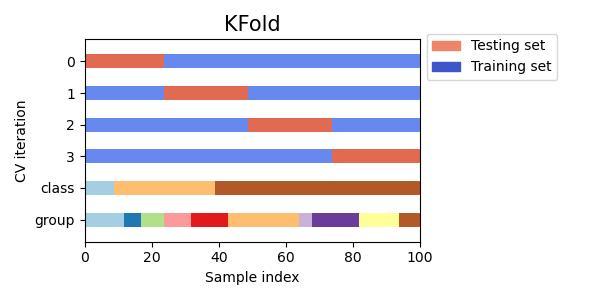
\includegraphics[width=\textwidth,height=5cm,keepaspectratio=true]{../src/resources/kfold.png}
        %                 \caption{
        %                   KFold Visualization from the scikit-learn documentation \cite{scikit-learn}.
        %                 }
        %                 \label{fig:kfold}
        %             \end{figure}
        %             \item \textbf{group-k-fold method}: Variation of k-fold designed for situations where the data has inherent groupings or dependecies that should be preserved in the train/test split. In this method, the data is divided into \textit{K} folds, then an additional constraint is imposed to ensure that data point from the same group are in the same fold. The fig:groupkfold shows an example of a group-k-fold split.
        %             \begin{figure}[H]
        %                 \centering
        %                 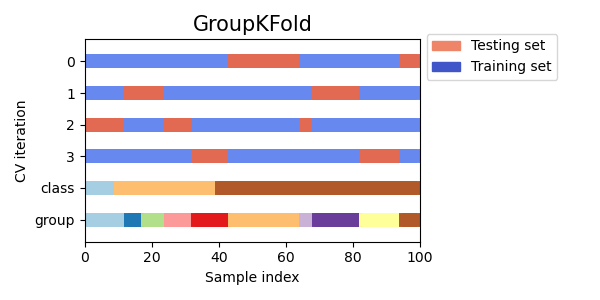
\includegraphics[width=\textwidth,height=5cm,keepaspectratio=true]{../src/resources/groupkfold.png}
        %                 \caption{
        %                   GroupKFold Visualization from the scikit-learn documentation \cite{scikit-learn}.
        %                 }
        %                 \label{fig:groupkfold}
        %             \end{figure}
        %         \end{itemize}
                
        % The advantage of using \textit{Cross-Validation} over \textit{Hold-Out} is that all the samples are used for both training and testing, and each sample is used for testing exactly once. This method helps to reduce the variance of the estimated performance of the model, by averaging the results over a number of trials. The disadvantage of using \textit{Cross-Validation} is that it is computationally expensive for very large datasets. \\ 

        % In this study, both methods are used to evaluate the performance of the models. The \textit{Hold-Out} method is used to evaluate the perfomance of the models for the \textit{Wrong approach} and \textit{Sequence approach} datasets due to their large dimension. The \textit{Cross-Validation} method is used toghether with the \textit{Hold-Out} method to evaluate the perfomance of the models for the \textit{Correct approach} and \textit{Feature Engineering approach} dataset due to them scoring the best results. 
        
        %* OK 
        \subsection{Metrics used}
            This section will report the metrics used to benchmark the different models used in this study.

            \subsubsection{Accuracy score}
                The \textit{accuracy} is the proportion of correct predictions, considering both true positives and true negatives, among the total number of samples. The formula used to calculate the accuracy is the following:
                \begin{equation}
                    \frac{TP + TN}{TP + TN + FP + FN}
                \end{equation} 
                where \textbf{TP} is the number of true positives, \textbf{TN} is the number of true negatives, \textbf{FP} is the number of false positives and \textbf{FN} is the number of false negatives.
            \subsubsection{Precision score}
                The \textit{precision} is the ability of the classifier not to label as positive a sample that is negative. The formula used to calculate the precision is the following:
                \begin{equation}
                    \frac{TP}{TP + FP}
                \end{equation}
            \subsubsection{Recall score}
                The \textit{recall} is the ability of the classifier to find all the positive samples. The formula used to calculate the recall is the following:
                \begin{equation}
                    \frac{TP}{TP + FN}
                \end{equation}
            \subsubsection{F1 score}
                The \textit{F1 score} is the harmonic mean of the precision and recall. The formula used to calculate the F1 score is the following:
                \begin{equation}
                    \frac{ 2 \times (precision \times recall)}{precision + recall}
                \end{equation}
            \subsubsection{Matthews correlation coefficent} 
                The \textit{Matthews correlation coefficent} (or $\varphi$ coefficient) takes into account true and false positives and negatives and is regarded as a balanced measure which can be used even if the classes are of very different sizes. The formula used to calculate the $\varphi$ coefficient is as follows: 
                \begin{equation}
                    \frac{TP \times TN - FP \times FN}{\sqrt{(TP + FP)(TP + FN)(TN + FP)(TN + FN)}}
                \end{equation}

            These metrics will be used to show the effectiveness of the approaches proposed in this thesis.
    
    % \section{Evaluation Results}
    %     TODO
    %     \subsubsection{Wrong Approach}

    %     This approach was the first one to be tested and it got surprisingly good results. Such a simple approach and yet high accuracy raised doubts about the validity of the results, after further investigation it was discovered that the dataset was not properly split into training and testing sets as stated 
        
        %! Wrong Approach
        % \begin{table}[htbp]
        %     \centering
        %     \begin{tabular}{lrrrrr}
        %         \toprule
        %         \textbf{Model} & \textbf{Accuracy} & \textbf{F1 Score} & \textbf{Recall} & \textbf{Precision} & \textbf{MCC} \\
        %         \midrule
        %         Random Forest & \textbf{0.9930} & \textbf{0.9914} & \textbf{0.9909} & \textbf{0.9919} & \textbf{0.9921} \\
        %         KNN& 0.9472 & 0.9369 & 0.9344 & 0.9400 & 0.9403 \\
        %         Decision Tree & 0.9364 & 0.9248 & 0.9240 & 0.9257 & 0.9280 \\
        %         SVM & 0.9313 & 0.9198 & 0.9190 & 0.9208 & 0.9223 \\
        %         Logistic Regression & 0.7902 & 0.7621 & 0.7599 & 0.7657 & 0.7623 \\
        %         \bottomrule
        %     \end{tabular}
        %     \caption{Evaluation results using \textbf{Hold-Out} validation method.}
        % \end{table}

        %\subsubsection{Sequence Approach}

        % This approach got the lowest results of all the approaches. This is due to the aggregate features function that is used to convert all sequences to the same dimension. This approach is not suitable for this type of data because it is losing a lot of information by aggregating the sequences. The results are shown in the table below.
        
        %! Sequence Approach
        % \begin{table}[htbp]
        %     \centering
        %     \begin{tabular}{lrrrrr}
        %         \toprule
        %         \textbf{Model} & \textbf{Accuracy} & \textbf{F1 Score} & \textbf{Recall} & \textbf{Precision} & \textbf{MCC} \\
        %         \midrule
        %         SVM & \textbf{0.5561} & \textbf{0.5045} & \textbf{0.5199} & \textbf{0.4937} & \textbf{0.5036} \\
        %         Random Forest & 0.4927 & 0.4567 & 0.4709 & 0.4894 & 0.4381 \\
        %         KNN & 0.4927 & 0.4857 & 0.4818 & 0.5121 & 0.4351 \\
        %         LogisticRegression & 0.4585 & 0.4655 & 0.4744 & 0.4730 & 0.3965 \\
        %         Decision Tree & 0.3756 & 0.3569 & 0.3694 & 0.3996 & 0.3100 \\
        %         \bottomrule
        %     \end{tabular}
        %     \caption{todo}
        % \end{table}

        %\subsubsection{Correct Approach}
        %! Correct Approach 
        % \begin{table}[ht]
        %     \centering
        %     \begin{tabular}{lrrrrr}
        %         \toprule
        %         \textbf{Model} & \textbf{Accuracy} & \textbf{F1 Score} & \textbf{Recall} & \textbf{Precision} & \textbf{MCC} \\
        %         \midrule
        %         Gradient Boosting & \textbf{0.6773} & \textbf{0.6574} & \textbf{0.6617} & \textbf{0.6595} & \textbf{0.6341} \\
        %         Support Vector Machine & 0.6538 & 0.6281 & 0.6370 & 0.6367 & 0.6093 \\
        %         LDA & 0.6362 & 0.6156 & 0.5987 & 0.6541 & 0.5905 \\
        %         KNN & 0.6292 & 0.5941 & 0.5971 & 0.5974 & 0.5788 \\
        %         Random Forest & 0.6257 & 0.6058 & 0.6239 & 0.6162 & 0.5793 \\
        %         MultiLayer & 0.5951 & 0.5731 & 0.5877 & 0.5931 & 0.5473 \\
        %         Naive Bayes & 0.5747 & 0.5576 & 0.5538 & 0.5980 & 0.5180 \\
        %         Logistic Regression & 0.5662 & 0.5175 & 0.5316 & 0.5215 & 0.5101 \\
        %         Decision Tree & 0.5224 & 0.4913 & 0.5001 & 0.5025 & 0.4618 \\
        %         AdaBoost & 0.3964 & 0.3026 & 0.3097 & 0.3733 & 0.3095 \\
        %         \bottomrule
        %     \end{tabular}
        %     \caption{todo}
        % \end{table}

        %! Cross-Validation vs Hold-Out in Correct Approach
        % \begin{table}[ht]
        %     \centering
        %     \begin{tabular}{lrrrrr}
        %         \toprule
        %         \textbf{Model} & \textbf{Accuracy} & \textbf{F1 Score} & \textbf{Recall} & \textbf{Precision} & \textbf{MCC} \\
        %         \midrule
        %         LDA (CV) & 0.6362 & 0.6169 & 0.6025 & 0.6732 & 0.5942 \\
        %         LDA (HO) & 0.6362 & 0.6156 & 0.5987 & 0.6541 & 0.5905 \\
        %         KNN (CV) & 0.6127 & 0.5832 & 0.5919 & 0.5917 & 0.5632 \\
        %         KNN (HO) & 0.6292 & 0.5941 & 0.5971 & 0.5974 & 0.5788 \\
        %         Naive Bayes (CV) & 0.5884 & 0.5551 & 0.5621 & 0.6176 & 0.5414 \\
        %         Naive Bayes (HO) & 0.5747 & 0.5576 & 0.5538 & 0.5980 & 0.5180 \\
        %         \bottomrule
        %         \end{tabular}
        %     \caption{CV = Cross-Validation, HO = Hold-Out}
        % \end{table}
        
        %! No mat walk vs no hoop walk - Correct Approach
        % \begin{table}[htbp]
        %     \centering
        %     \begin{minipage}{\linewidth}
        %         \centering
        %         \begin{tabular}{lrrrrr}
        %             \toprule
        %             \textbf{Model} & \textbf{Accuracy} & \textbf{F1 Score} & \textbf{Recall} & \textbf{Precision} & \textbf{MCC} \\
        %             \midrule
        %             Gradient Boosting & \textbf{0.7137} & \textbf{0.7059} & \textbf{0.7133} & \textbf{0.7048} & \textbf{0.6711} \\
        %             SVM & 0.7024 & 0.6860 & 0.6976 & 0.6909 & 0.6594 \\
        %             LDA & 0.6933 & 0.6829 & 0.6725 & 0.7233 & 0.6513 \\
        %             \bottomrule
        %         \end{tabular}
        %         \caption{Table 1}
        %         \vspace{5pt} 
        
        %         \begin{tabular}{lrrrrr}
        %             \toprule
        %             \textbf{Model} & \textbf{Accuracy} & \textbf{F1 Score} & \textbf{Recall} & \textbf{Precision} & \textbf{MCC} \\
        %             \midrule
        %             SVM & \textbf{0.7073} & \textbf{0.6908} & \textbf{0.6984} & \textbf{0.6942} & \textbf{0.6630} \\
        %             LDA & 0.6890 & 0.6732 & 0.6651 & 0.7039 & 0.6452 \\
        %             Gradient Boosting & 0.6887 & 0.6798 & 0.6866 & 0.6817 & 0.6421 \\
        %             \bottomrule
        %         \end{tabular}
        %         \caption{Table 2}
        %     \end{minipage}
        % \end{table}

    %\subsubsection{Feature Engineering Approach}
        %! Feature Engineering Approach
        % \begin{table}[ht]
        %     \centering
        %     \begin{tabular}{lrrrrr}
        %         \toprule
        %         \textbf{Model} & \textbf{Accuracy} & \textbf{F1 Score} & \textbf{Recall} & \textbf{Precision} & \textbf{MCC} \\
        %         \midrule
        %         MLP & \textbf{0.8291}& \textbf{0.8375} & \textbf{0.8426} & \textbf{0.8472} & \textbf{0.8111} \\
        %         LDA & 0.8217 & 0.8125 & 0.8183 & 0.8298 & 0.8040 \\
        %         Logistic Regression & 0.8094 & 0.8063 & 0.8168 & 0.8292 & 0.7915 \\
        %         Random Forest & 0.8024 & 0.8146 & 0.8176 & 0.8255 & 0.7812 \\
        %         Gradient Boosting & 0.7766 & 0.7849 & 0.7878 & 0.8063 & 0.7530 \\
        %         SVM & 0.7631 & 0.7613 & 0.7802 & 0.7888 & 0.7428 \\
        %         KNN & 0.7485 & 0.7590 & 0.7656 & 0.7758 & 0.7221 \\
        %         Decision Tree & 0.7019 & 0.7069 & 0.7225 & 0.7175 & 0.6713 \\
        %         Naive Bayes & 0.6808 & 0.6833 & 0.7036 & 0.7245 & 0.6510 \\
        %         AdaBoost & 0.3869 & 0.3225 & 0.3970 & 0.3421 & 0.3465 \\
        %         \bottomrule
        %     \end{tabular}
        %     \caption{todo}
        % \end{table}

        %! Feature Engineering Approach - Hold-Out
        % \begin{table}[ht]
        %     \centering
        %     \begin{tabular}{lrrrrr}
        %         \toprule
        %         \textbf{Model} & \textbf{Accuracy} & \textbf{F1 Score} & \textbf{Recall} & \textbf{Precision} & \textbf{MCC} \\
        %         \midrule
        %           LDA (HO) & 0.8049 & 0.8094 & 0.8085 & 0.8140 & 0.7823 \\
        %           LDA (CV) & 0.8217 & 0.8125 & 0.8183 & 0.8298 & 0.8040 \\
        %           Logistic Regression (HO) & 0.8000 & 0.8111 & 0.8141 & 0.8157 & 0.7777 \\
        %           Logistic Regression (CV) & 0.8094 & 0.8063 & 0.8168 & 0.8292 & 0.7915 \\
        %           Random Forest (HO) & 0.7805 & 0.7947 & 0.7936 & 0.8033 & 0.7558 \\
        %           Random Forest (CV) & 0.8024 & 0.8146 & 0.8176 & 0.8255 & 0.7812 \\
        %         \bottomrule
        %         \end{tabular}
        %     \caption{CV = Cross-Validation, HO = Hold-Out}
        % \end{table}

        %! No mat walk vs no hoop walk - Correct Approach
        % \begin{table}[htbp]
        %     \centering
        %     \begin{minipage}{\linewidth}
        %         \centering
        %         \begin{tabular}{lrrrrr}
        %             \toprule
        %             \textbf{Model} & \textbf{Accuracy} & \textbf{F1 Score} & \textbf{Recall} & \textbf{Precision} & \textbf{MCC} \\
        %             \midrule
        %             LDA & \textbf{0.9310} & \textbf{0.9257} & \textbf{0.9256} & \textbf{0.9420} & \textbf{0.9232} \\
        %             MLP & 0.9093 & 0.9121 & 0.9131 & 0.9245 & 0.8989 \\
        %             Logistic Regression & 0.9040 & 0.9010 & 0.9016 & 0.9235 & 0.8937 \\
        %             \bottomrule
        %         \end{tabular}
        %         \caption{Mat-Walk movement data removed from the dataset.}
        %         \vspace{5pt} 
        %         \begin{tabular}{lrrrrr}
        %             \toprule
        %             \textbf{Model} & \textbf{Accuracy} & \textbf{F1 Score} & \textbf{Recall} & \textbf{Precision} & \textbf{MCC} \\
        %             \midrule
        %             LDA & \textbf{0.9421} & \textbf{0.9407} & \textbf{0.9403} & \textbf{0.9515} & \textbf{0.9353} \\
        %             MLP & 0.9206 & 0.9269 & 0.9278 & 0.9365 & 0.9115 \\
        %             Logistic Regression & 0.9119 & 0.9181 & 0.9191 & 0.9292 & 0.9019 \\
        %             \bottomrule
        %         \end{tabular}
        %         \caption{Hoop-Walk movement data removed from the dataset.}
        %     \end{minipage}
        % \end{table}
    
    \section{Comparative Analysis}
        
    \section{Discussion of Key Findings}

\cleardoublepage